\documentclass{iitsrc}
\usepackage{graphicx}
\usepackage{mflogo}
\usepackage{courier}
\usepackage[utf8]{inputenc}

\title{StumbleUpon Evergreen Classification Challenge}
\titlerunning{StumbleUpon Evergreen Classification Challenge}
\author{Liščák}{Tomáš}
\author{Makan}{Branislav}
\supervision{~\ms}
            {\infosys~}
            {Ing.~Róbert Móro}
            {~\iiisse, \fiit}

\begin{document}
\maketitle

\begin{multicols}{2}
\raggedcolumns

\section{Opis problému}
Odporúčajúci systém StumbleUpon odporúča svojim užívateľom stránky, pričom si potrpí na vysokej kvalite týchto stránok. Kvalita stránky je aj to, či bude stabilná, alebo dlhodobo úspešná. Takéto ``evergreen`` stránky sa bežne zisťujú skrz používateľskú odozvu, avšak problémom je ako tento údaj vedieť ešte predtým, než je stránka vôbec hocikomu odporúčaná. Existuje predpoklad, že určité vlastnosti stránky by mohli indikovať, či má stránka potenciál na to byť ``evergreen``. Ak by sa dali tieto vlastnosti odhaliť, dal by sa vytvoriť klasifikátor, ktorý za ich využitia takto stránku korektne zaradí. Práve preto je toto úloha pre strojové učenie , konkrétne aplikovanie klasifikátora na zvolené atribúty, ktorou sa budeme zaoberať v našom projekte.

\section{Opis dát}
Ako zdrojov dát je dostupných niekoľko súborov vo formáte tsv, angl. ``tab-separated values``. Prvý zhluk týchto skomprimovaných súborov predstavujú obsahy jednotlivých stránok zapísané v tomto formáte. Ako názvy súborov sú uvedené ID stránok.

Ďalšie dva tsv súbory sú nazvané train a test, pretože je jeden určený pre trénovanie, obsahujúci 7395 stránok, a druhý pre testovanie, obsahujúci 3171 stránok. Tieto súbory obsahujú meta-údaje o stránkach, obsahujúce niekoľko atribútov:

\begin{itemize}
	\item \emph{Url stránky} a \emph{ID stránky}, ktoré je rovnaké ako názov súboru obsahujúceho obsah danej stránky v zhluku komprimovaných tsv súborov.
	\item \emph{Boilerplate}, obsahujúci krátky opis stránky v json formáte.
	\item \emph{Alchemy kategória a skóre} z verejne dostupného ohodnocovača stránok Alchemy API.
	\item \emph{Veľkostné údaje}, medzi ktoré patria priemerný počet slov na linku stránky, celkový počet textových slov a počet tagov, ako sú: \mbox{\textless embed \textgreater}, \mbox{\textless a \textgreater}.
	\item \emph{Pomerové údaje}, medzi ktoré patria podobnosť odkazov počítaná percentom odkazov obsahujúcich 1,2,3, alebo 4 podobné slová, dosiahnutá kompresia (pomer redundantných informácií), pomer \mbox{\textless iframe \textgreater} tagov voči celkovému počtu tagov, pomer tagov voči textu, pomer \mbox{\textless img \textgreater} tagov voči textu, percento slov na stránke, ktoré nie sú súčasťou linku a nakoniec pomer slov nenájdených vo wiki (chybne napísaných).
	\item \emph{Príznakové údaje}, medzi ktoré patria príznak, či má stránka \mbox{\textless frame \textgreater} tag, ale nemá žiadny \mbox{\textless body \textgreater} tag, príznak, či stránka obsahuje doménový odkaz s tagom \textless a \textgreater, príznak, či je stránka klasifikovaná StumbleUpon klasifikátorom ako správa, alebo správa na titulnej strane, príznak, že aspoň 3 odkazy obsahujú viac ako 30 alfanumerických znakov a nakoniec pre trénovaciu množinu príznak, či je stránka ``evergreen``, alebo nie.
\end{itemize}

\section{Predspracovanie atribútov}
Pre dané atribúty sme spravili štatistickú analýzu, na základe ktorej sa odfiltruje podmnožina dimenzií, ktoré budú predstavovať vstupné údaje do klasifikátora. Pri filtrácii sme zohľadnili chýbajúce údaje, logickú použiteľnosť každého atribútu pre klasifikačnú úlohu a korelačné vzťahy každého s každým atribútom. Výsledné vyradené atribúty sú:

\begin{itemize}
	\item \emph{Embed Ratio} atribút obsahuje hodnoty, ako výsledky pomeru, so silným zastúpením hodnôt -1 a 0 (6900 hodnôt z 7395), pričom zvyšné hodnoty sú v rozsahu 0 - 0.2. Na koľko nepoznáme interpretáciu týchto hodnôt a zdá sa nám, že pomer zmysluplných hodnôt je príliš malý, je tiež tento atribút vyradený.
	\item \emph{Frame Based} nezohľadňujeme kvôli tomu, že obsahuje samé nuly a je to teda pokazený atribút.
	\item Zvyšné 3 atribúty \emph{commonlink\_ratio} boli odstránené na základe ich silnej korelácie.
\end{itemize}

Ostatné atribúty vidíme ako potencionálne použiteľné pre klasifikátor. Zostávajúce atribúty však bolo nutné predspracovať a to \emph{doplnením chýbajúcich údajov, odstránením odľahlých hodnôt a normalizáciou}.

V rámci tohto predspracovania atribútov sa:

\begin{itemize}
	\item doplnili nuly do chýbajúcich hodnôt atribútu \emph{News Front Page}, nakoľko je prevažná väčšina hodnôt 0, indikujúca, že stránka nie je novinárska, čo je tiež vo všeobecnosti prípad väčšiny stránok,
	\item odstránili odľahlé hodnoty v atribúte \emph{Image Ratio} okresaním hodnôt na interval 0-1, pričom za chybné hodnoty boli doplnené priemerné hodnoty
	\item a nakoniec sa normalizovali všetky zvyšné numerické atribúty na rozsah 0 - 1 rovnicou:
	\begin{equation}
	(x - min)/(max - min)
	\end{equation}
	čo bolo potrebné pri vkladaní atribútov ako vstupov do neurónovej siete.
\end{itemize}

\subsection{Textový obsah}
Posledným a aj najpracnejším atribútom pre predspracovanie je textový obsah webových stránok – tzv. surové dáta (raw data). Tieto dáta sú uložené v JSON (JavaScript Object Notation) formáte. Rozdelené sú na tri časti: titul (title), body (textový obsah stránky) a url stránky. Práve samotný textový obsah je z týchto najzaujímavejší.

Textový obsah sa najprv normalizuje. V rámci normalizácie sa vykonajú nasledovné operácie:

\begin{itemize}
	\item Transformácia textu do malých písmen (lowercase).
	\item Odstránenie všetkých ne-písmenkových znakov.
	\item Alternatívne sa po potrebe koná aj lamatizácia a stemovanie textu. Lematizácia je určenie základného (slovníkového) tvaru slova, tzv. lemy \cite{fiittext}.
\end{itemize}
%
Táto forma normalizácie je vhodná na analýzu obsahu textu, napr. kľúčové slová, alebo tému textu.

Základnou formou pri väčšine techník na spracovanie textových dát je dátová štruktúra vrece slov (ang. bag of words). Takéto vrece obsahuje všetky unikátne slová zo vstupného dokumentu. Okrem samotného vreca slov, počítame aj frekvenciu výskytu jednotlivých slov v dokumente a lexikálnu rôznorodosť dokumentu – pomer medzi počtom unikátnych slov a celkovým počtom slov v dokumente.

V rámci spracovania textového obsahu sme sa zamerali na určovanie témy, resp. kategórie, či žánru textu, napr. či je text o zdraviu, politiky alebo športe a podobne. Tejto problematike sa hovorí klasifikácia dokumentu. Dva základné prístupy ku klasifikácii dokumentov sú klasifikácia s učiteľom a bez učiteľa (supervised and unsupervised classification).

Hlavným problémom klasifikácie s učiteľom je nedostatok vhodných voľne dostupných oanotovaných textových datasetov. Z tohto dôvodu sme sa rozhodli využiť dáta, ktoré máme k dispozícii. Zhruba 70\% záznamov majú určenú kategóriu textového obsahu – atribút alchemy category. Natrénovaním klasifikátora na týchto dátach sa môžu jednotlivé kategórie priradiť všetkých textom. Na tento účel sme sa rozhodli použiť najpoužívanejší modul na analýzu textu NLTK (Natural Language Toolkit) pre Python. Tento ponúka naivný Baiesov klasifikátor a rozhodujúce stromy. Oba si však vyžadujú ukladanie slov do pythonovkých slovníkov, ktoré pri našich textových dátach dosiahli veľkú pamäťovú náročnosť – na notebooku s veľkosťou RAM pamäte 12 GB nám zmrzol celý operačný systém po asi desiatich minútach behu skriptu.

Analýza textových dát je celkom obsiahla téma sama o sebe. Zatiaľ sa nám nepodarilo extrahovať témy z textových dát, no stále máme na pláne sa týmto zaoberať a v neskoršej fáze pridáme spracované textové dáta ku kalsifikačnému modelu. Po konzultácii s viac skúsenými kolegami, rozhodli sme sa vyskúšať modul \emph{scikit-learn}, pomocou ktorého budeme extrahovať témy z textových dát.

Klasifikáciu bez učiteľa na extrahovanie tém sme zatiaľ nevyskúšali. V prípade, že sa nám nebude dariť s riadenou klasifikáciou, vyskúšame neriadenú.

\section{Stručný opis prác iných autorov}
Po vyhľadávaní nášho typu problému vo vedeckej literatúre sme narazili najbližšie na klasifikáciu kategórie stránok na základe jej obsahu \cite{kosala2000web}, čo však nie je náš hlavný problém a týka sa len vedľajšej úlohy doplnenia chýbajúcich údajov o kategóriách stránok. Povahou nášho klasifikátora je učenie sa na základe istých numerických čŕt, ako meta-údajov stránok, na čo nám je hlavne treba vedieť typy klasifikátorov a ich vhodnosť použitia v daných situáciách \cite{qi2009web}.  Na tomto základe sme sa rozhodli použiť neurónové siete, ktorých princípy a typy sietí sme si dôkladne preštudovali v článkoch \cite{de1997brief} a \cite{lek1999artificial}.

\section{Modely dolovania dát}
Našim výstupom je model klasifikátora, ktorý je schopný určiť ``evergreen`` vlastnosť stránky s čo najvyššou úspešnosťou, pričom sa takto tiež získajú znalosti o tom, ktoré atribúty webových stránok najviac na túto vlastnosť vplývajú.

Na túto úlohu je vhodných viacero ``supervised`` klasifikátorov, ktoré sme zohľadňovali:

\begin{itemize}
	\item Rozhodovacie stromy - trom pravidiel, nevýhodou slabšia presnosť, výhodou vyššia rýchlosť.
	\item Support vector machines - Nová, úspešná metóda, avšak väčšia pracnosť s predspracovaním atribútov nelineárne pôsobiacich na výsledný atribút.
	\item Neurónové siete - nie je vidno ``do vnútra`` výpočtov siete a takisto je potreba korektne nastaviť veľké množstvo atribútov, avšak dosahujú veľmi vysokú úspešnosť.
	\item Bayersovské siete - siete rovníc pravdepodobností, aplikačne podobné neurónovým sieťam.
\end{itemize}

Po zvážení metód sme sa nakoniec rozhodli pre neurónové siete, nakoľko jednak dosahujú veľmi vysokú úspešnosť a jednak existuje množstvo rôznych typov, ktoré ponúkajú rôzne knižnice, ktoré sa dajú využiť a odskúšať ich vhodnosť na tento typ úlohy. Budeme sa preto snažiť zahrnúť čo najväčšiu škálu typov sietí a nastavených parametrov, aby sme prišli na tú najvhodnejšiu kombináciu a dosiahli tak najlepší výsledok. Vhodnou voľbou by boli aj bayersovské siete, avšak z časového hľadiska sa uvidí, či otestujeme a porovnáme aj úspešnosť tohto modelu na tejto úlohe.

\section{Prvotné experimenty}
Spočiatku sme chceli vybrať knižnice, ako sú keras staviaci na tensorflow a neupy, avšak obe knižnice sa nepodarilo ani vyskúšať, kvôli problémom s inštaláciou ``dependencies``. Nakoniec sme ako zvolenú knižnicu pre neurónovú sieť vybrali \emph{NeuroLab} pre python, z dôvodu nekonfliktnej inštalácie a takisto ponuky veľa rôznych typov sietí a intuitívneho nastavovania parametrov.

V rámci prvotných experimentov sme si pripravili vstupné a učiace trénovacie a testovacie dáta z predspracovaných dataframov a vložili sme ich do multi-vrstvového perceptrónu s troma vrstvami neurónov (5-5-1) na trénovanie a testovanie. Vstupné trénovacie obsahovali len 5 náhodne zvolených atribútov a len 100 záznamov, pretože nám šlo o prvotné otestovanie funkcionality siete a zoznámene sa s knižnicou.

\begin{figure}[H]
    \begin{center}
        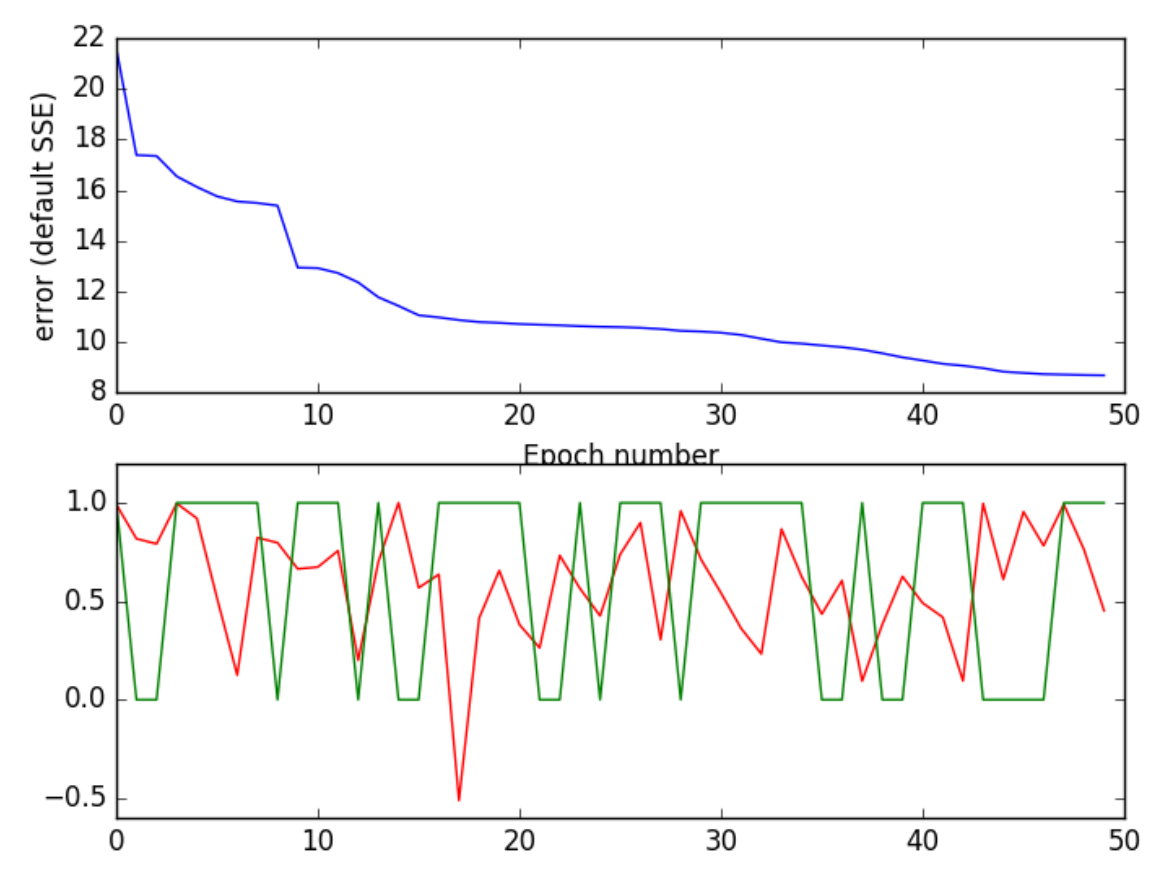
\includegraphics[width=\linewidth]{results}
        \caption{Klesajúca chyba klasifikácie pri trénovaní siete a výstup siete v porovnaní s reálnymi hodnotami pre testovacie dáta.}
    \end{center}
\end{figure}

Testovacie dáta obsahovali 50 záznamov a na spodnom obrázku je vidno výstup siete červenou farbou a reálne hodnoty pre testovacie dáta zelenou farbou. Na vrchnom obrázku je zasa vidno klesajúca chyba klasifikácie pri trénovaní siete pre 50 epóch.

Parametre MLP(multi layered perceptron) sú aktivačná funkcia neurónov, počet epóch, cieľová úspešnosť  a  algoritmus učenia. Možnými voľbami pre algoritmus učenia sú napr. \emph{simple gradient descent backpropagation, gradient descent with momentum, gradient descent with adaptive learning rate a resilient backpropagation}, pričom u každého spôsobu je možné nastaviť veľa parametrov ako sú momentum, maximálna a minimálna zmena váhy, learning rate atď.

Ďalšie možné typy sietí sú \emph{kohonenove siete, elmanove rekurentné siete, hammingove rekurentné siete, hopfieldové rekurentné siete a learning vector qantization} sieť z ktorých sa určite budú dať niektoré ďalšie vyskúšať pre túto úlohu.

\section{Vyhodnocovanie}
Ako vyhodnocovaciu mieru sa bežne používa chyba klasifikácie, čo je normalizovaná suma štvorcov rozdielov medzi klasifikovanou a korektnou hodnotou. V súčasne používanej knižnici NeuroLab má každý typ siete pri trénovaní priradený iný typ počítania chyby, ako je to napr. pri MLP chyba SSE(suma štvorcov chýb), avšak pri vyhodnocovaní modelu sa kvôli porovnateľnosti prístupov explicitne vytvorí funkcia na rátanie normalizovanej chyby, ako je MAPE, alebo MSE.

V rámci grafov použijeme zobrazenie testovacieho výstupu oproti sieťou vypočítaného výstupu, pričom takisto môžeme použiť ROC krivku vzhľadom na mieru presnosti a špecifickosti klasifikácie.

% Please do not remove this.
\let\OLDthebibliography\thebibliography
\renewcommand\thebibliography[1]{
  \OLDthebibliography{#1}
  \setlength{\parskip}{5pt}
 \footnotesize
}

\bibliography{literature}
\bibliographystyle{iitsrc}

\end{multicols}
\end{document}
